\chapter{Stand van zaken}
\label{ch:stand-van-zaken}

% Tip: Begin elk hoofdstuk met een paragraaf inleiding die beschrijft hoe
% dit hoofdstuk past binnen het geheel van de bachelorproef. Geef in het
% bijzonder aan wat de link is met het vorige en volgende hoofdstuk.

% Pas na deze inleidende paragraaf komt de eerste sectiehoofding.

\section{Inleiding}

In dit hoofstuk zal er een stand van zaken gegeven worden van het onderwerp, hoe het vroeger gebeurde en hoe het tegenwoordig gebeurt. In sectie \ref{sec:NFC} zal een korte uitleg gegeven worden over NFC technologie. Sectie \ref{sec:HCE} wordt besproken hoe het simuleren van draadloze smart cards gebeurt. 
Sinds de komst van Android 4.4 oftewel Android KitKat introduceerde Google een nieuwe technologie genaamd Host-based Card Emulation (HCE). HCE technologie maakt het mogelijk om Near Field Communication (NFC) technologie te gebruiken zonder de aanwezigheid van een secure element. 
Wanneer het Android toestel zich in card emulation (CE) mode bevindt en tegen een draadloze leer of point-of-sale (POS) terminal gehouden wordt, heeft het toestel de mogelijkheid om allerhande soorten draadloze smart cards te simuleren. Deze contactloze smart cards worden in vele situaties gebruikt zoals bij draadloos betalen, loyalty systemen, ticketing, toegang tot gebouwen,... ~\autocite{SCA2014}.

\section{Near Field Communication (NFC)}
\label{sec:NFC}
Near Field Communication (NFC) is een technologie die communicatie vanop korte afstanden, meestal nul tot vier centimeter maar kan tot 20 centimeter oplopen, mogelijk maakt. NFC apparaten kunnen actief of passief zijn, wanneer het NFC apparaat actief is dan gebruikt dit apparaat zijn eigen energiebron om zijn radio frequentie te genereren. Een passief NFC apparaat gebruikt de energiebron van een actief NFC apparaat om data te versturen, passieve NFC apparaten kunnen ook enkel maar antwoorden op aanvragen die vanaf een actief NFC apparaat verstuurd wordt. Transacties worden automatisch gestart door twee NFC apparaten elkaar te laten raken of deze twee dicht bij elkaar te houden ~\autocite{Alattar2014}. 

NFC heeft drie verschillende operating modes: Peer to Peer mode, Reader/Writer mode en Contactless Card Emulation. Peer To Peer mode biedt de mogelijkheid om data te versturen tussen twee NFC apparaten aan snelheden tot 424 Kbit/s. Reader/Writer mode maakt het mogelijk dat twee NFC apparaten gebruikt kunnen worden voor het lezen/schrijven van tags en draadloze smart cards, hierbij is de snelheid van het versturen van de data maar 106 Kbit/s. Contactless Card Emulation laat de NFC apparaten draadloze smart cards of tags simuleren die gelezen of naar geschreven kunnen worden door een NFC lezer ~\autocite{Alattar2014}. 

\section{Host-based Card Emulation (HCE)}
\label{sec:HCE}
HCE maakt het dus mogelijk voor NFC apparaten om draadloze smart cards te simuleren. Om gebruik te kunnen maken van HCE heeft android verschillende libraries en APIs (Application Programming Interface) geimplementeerd in het besturingssysteem. Deze libraries en APIs worden overschreven door de applicaties die hier gebruik van willen maken en die op de CPU van het apparaat draaien, deze applicaties kunnen dan APDU (Application Protocol Data Unit) commando's en antwoorden uitwisselen met een NFC POS. Wanneer men vroeger gebruik wou maken van de NFC technologie kon dit alleen door een Secure Element (SE) die ingebouwd zat in het apparaat zoals een SIM kaart. De applicaties werden geïnstalleerd op dit SE die dan de APDU's afhandelde om zo draadloze smart cards veilig te kunnen simuleren. De APDU's die verstuurd worden van een NFC lezer worden opgevangen door de NFC antenne van het appparaat en wordt doorgegeven via de NFC controller naar het SE en omgekeerd zie figuur. Met HCE is het de bedoeling dat de nood van een SE verwijdert wordt uit deze operatie, ipv de APDU's door te geven naar het SE worden deze door gegeven naar de CPU van het apparaat en omgekeerd zie figuur ~\ref{fig:SE-HCE} ~\autocite{Alattar2014}. 

\begin{figure}
	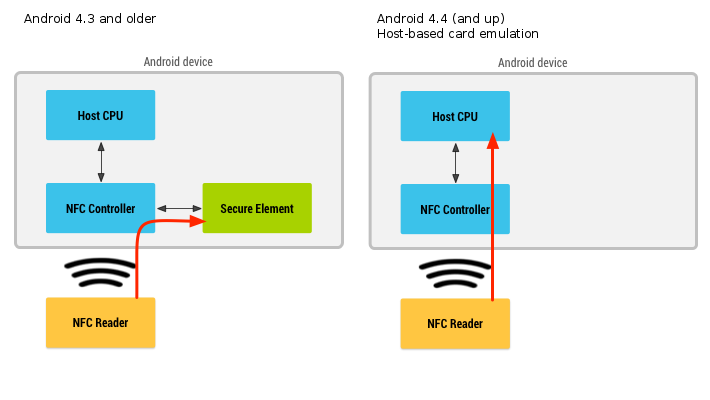
\includegraphics[width=\linewidth]
	{img/WalletHostBasedCardEmulation}
	\caption{Simulatie van een smart card via SE}
	\label{fig:SE-HCE}
\end{figure}
